\documentclass{report}
\usepackage{caption}
\usepackage{subcaption}
\usepackage[T1]{fontenc}
\usepackage[utf8]{inputenc}
\usepackage{import}
\usepackage[english]{babel}
\usepackage{minted}
\usepackage{tikz}
\usepackage{amsmath}
\usepackage{amsthm}
\usepackage{cleveref}
\usepackage{tabularray}
\usepackage{tabularx}
\usepackage{biblatex}
\usepackage{multirow}
\usetikzlibrary{graphs}
\usetikzlibrary{trees}
\usepackage{xcolor}
\usepackage{array}
%\newcolumntype{C}[1]{>%{\centering\arraybackslash}p{#1}}
\addbibresource{bbl.bib}
\newtheorem{theorem}{Theorem}
\newtheorem{definition}{Definition}
\begin{document}
\begin{titlepage}
\begin{center}        
	\large
	\textbf{Jagiellonian University}\\
	Department of Theoretical Computer Science\\

	\vspace{1.5cm}

	\Large
	\textbf{Rafał Kilar}

	\vspace*{2cm}

	\textbf{\LARGE Comparison of maximum weight matching algorithms on general graphs}
	
	\vspace{0.5cm}
	\large
	
	\vfill
	\Large
	Master's Thesis

	\vfill
	\Large
	Supervisor: dr hab. in\.z. Krzysztof Turowski
	
	\vspace{0.8cm}
	
	September 2024
\end{center}
\end{titlepage}

\pagebreak
\tableofcontents

\pagebreak
\chapter{Introduction}
The graph matching problem is among the most extensively researched topics in combinatorial optimization. Initial studies into the subject were motivated by practical issues including minimization of transportation costs~\cite{hitchcock1941distribution} or optimally assigning personnel to tasks~\cite{thorndike1950problem}. Over time, matching algorithms have found their use in scheduling, approximation algorithms and network switching among other problems. They play a crucial role in various other optimization algorithms including undirected shortest paths~\cite{lawler2001combinatorial}, planar maximum cut~\cite{hadlock1975finding}, metric traveling salesman problem~\cite{christofides2022worst}, and Chinese postman tours~\cite{edmonds1973matching}.

\section{Definitions}

We first give some basic definitions in graph theory sourced from~\cite{bollobás1998modern}.

\begin{defn}[graph]
    A \emph{graph} $G$ is an ordered pair of disjoint sets $(V, E)$ such that $E$ is a subset of the set $V \choose 2$ of unordered pairs of $V$. 
\end{defn}

We only consider finite graphs, that is, $V$ and $E$ are always finite. The set $V$ is the set of \emph{vertices} and $E$ is the set of \emph{edges}. If $G$ is a graph, then $V = V(G)$ is the \emph{vertex set} of $G$, and $E = E(G)$ is the \emph{edge set} of $G$. If $v$ is a vertex of $G$ we will sometimes write $v \in G$ instead of $v \in V(G)$. 

We denote $n_G = |V(G)|$ and $m_G = |E(G)|$ for a graph $G = (V, E)$. We will drop the subscripts for brevity when $G$ is clear from the context.

An edge $\{ x, y \}$ is said to \emph{join} the vertices $x$ and $y$ and is denoted $xy$. Thus, $xy$ and $yx$ mean exactly the same edge, the vertices $x$ and $y$ are the \emph{endvertices} of this edge. If $xy \in E(G)$, then $x$ and $y$ are \emph{adjacent}, \emph{neighboring} or \emph{connected}, and the  vertices $x$ and $y$ are \emph{incident} with the edge $xy$. Two edges are \emph{adjacent} if the have exactly one common endvertex.

The set of vertices adjacent to a vertex $v \in G$.

\begin{defn}[subgraph]
    We say that $G' = (V', E')$ is a \emph{subgraph} of $G = (V, E)$ if $V' \subseteq V$ and $E' \subseteq E$. In this case we write $G' \subseteq G$. If $G'$ contains all edges of $G$ that join two vertices in $V'$ then $G'$ is said to be a subgraph \emph{induced} or \emph{spanned} by $B'$ and is denoted $G[V']$. 
\end{defn}

For a subgraph $G' = G[H]$ spanned by a vertex subset $H \subseteq V(G)$, we write $n_H = |H|$ and $m_H = |E(G')|$.

If $W \subseteq V(G)$, then $G - W = G[V \setminus W]$ is the subgraph of $G$ obtained by deleting the vertices of $W$ and all edges incident with them. Similarly, if $E' \subseteq E(G)$, then $G - E' = (V(G), E(G) \setminus E')$. If $W = \{ w \}$ and $E' = \{ xy \}$ for some vertex $w \in V(G)$ and edge $xy \in E(G)$, then the notation is simplified to $G - w$ and $G - xy$. Similarly, if $x$ and $y$ are nonadjacent vertices of $G$, then $G + xy = (V(G), E(G) \cup \{ xy \})$.

\begin{defn}[path]
    A \emph{path} is a graph $P$ of the form

    \begin{align*}
        V(P) &= \{x_0, x_1, \dots, x_l\} \\
        E(P) &= \{x_0x_1, x_1x_2, \dots, x_{l-1}x_l\}
    \end{align*}
\end{defn}

This path $P$ is usually denoted by $x_0x_1\dots x_l$. The vertices $x_0$ and $x_l$ are the \emph{ends} of $P$ and the value $l = |E(P)|$ is the \emph{length} of $P$. We say that $P$ goes from $x_0$ to $x_l$.

\begin{defn}[connected graph]
    A graph is \emph{connected} if for every pair $\{x, y\}$ of distinct vertices there is a path from $x$ to $y$.
\end{defn}

A maximal connected subgraph is a \emph{component} of a graph.

\begin{defn}[cycle]
    A \emph{cycle} is a graph $C$ of the form

    \begin{align*}
        V(C) &= \{x_0, x_1, \dots, x_l\} \\
        E(C) &= \{x_0x_1, x_1x_2, \dots, x_{l-1}x_l, x_l x_0\}
    \end{align*}
\end{defn}

This cycle $C$ is denoted by $x_0 x_1\dots x_l x_1$. The value $l + 1 = |E(C)| = |V(C)|$ is the \emph{length} of $C$. 

\begin{defn}[forest, tree]
    A graph without any cycles is a \emph{forest}, or an \emph{acyclic} graph. A \emph{tree} is connected forest.
\end{defn}

\begin{defn}[bipartite graph]
    A graph $G$ is a \emph{bipartite} graph with vertex classes $V_1$ and $V_2$ if $V(G) = V_1 \cup V_2$, $V_1 \cap V_2 = \emptyset$ and every edge joins a vertex of $V_1$ to a vertex of $V_2$.
\end{defn}

An easy observation is that a graph is bipartite if and only if it does not contain an odd-length cycle.

A set of vertices (edges) is \emph{independent} if no two elements of it are adjacent.

\begin{defn}[matching]
    A set of independent edges is called a \emph{matching}. A matching $M$ is \emph{perfect} if every vertex is adjacent to exactly one edge in $M$.
\end{defn}

\begin{defn}[matched vertex/edge]
    A vertex $v$ is \emph{exposed} for a matching $M$ if it's not adjacent to any edge in $M$. If a vertex is not exposed it is \emph{matched}. Similarly, we say that an edge $e$ is \emph{matched} if $e \in M$.
\end{defn}

If a vertex $v$ is matched in a matching $M$, then we call the vertex $u$, such that $uv \in M$, the \emph{mate} or \emph{matched vertex} of $v$.

\begin{defn}[alternating path]
    A path $P = x_0x_1\dots x_l$ is alternating for a matching $M$ if for each $i \in \{0, \dots, l - 2\}$, $x_i x_{i+1} \in M$ if and only if $x_{i+1}x_{i+2} \notin M$.
\end{defn}

\begin{defn}[augmenting path]
    An alternating path $x_0x_1\dots x_l$ is \emph{augmenting} if the vertices $x_0$ and $x_l$ are both exposed.
\end{defn}

\begin{defn}[weighted graph]
    A \emph{weighted} graph is a graph $G = (V, E)$ along with a \emph{weight function} $w : E \rightarrow \mathbb{R}$, which assigns a real valued \emph{weight} $w(e)$ to each edge of $G$.
\end{defn}

For a set of edges $S \subseteq E$, we define the \emph{weight} of $S$ to be $w(S) = \sum_{e \in S} w(e)$. 

We denote $N_G = \max_{e \in E} w(e)$ for a graph $G = (V, E)$, which we shorten to $N$ when $G$ is clear from the context. In this work, we consider only graphs with non-negative weights.

The algorithms for the maximum matching problems are usually divided into groups based on the classes of graphs they operate on and the type of matching they find. The graphs can be either bipartite or non-bipartite. When the graphs are unweighted, the algorithms find matchings with maximum number of edges. When they're weighted, a matching with maximum possible weight is sought. In the case of weighted graphs we can also restrict our search to perfect matching, looking for the one with the highest weight. In this work we consider the following variants of the maximum matching problem on general graphs:

\begin{itemize}
    \item \textsc{Maximum Cardinality Matching} (\textsc{MCM}) Find a matching in a graph $G$ with maximum number of edges,
    \item \textsc{Maximum Weight Matching} (\textsc{MWM}) Find a matching in a weighted graph $G$ with maximum weight,
    \item \textsc{Maximum Weight Perfect Matching} (\textsc{MWPM}) Find a perfect matching in a weighted graph $G$ with maximum weight.
\end{itemize}

\begin{theorem}\label{thm:reduction}
The \textsc{MWM} and \textsc{MWPM} problems are reducible to each other.

\begin{proof}
    For an instance $G=(V, E)$ of \textsc{MWM}, define a new graph $G' = (V', E')$ where $V' = V_1 \cup V_2$ consists of two copies of $V$ and the edge set $E'$ contains two copies of $E$ along with zero-weight edges between each corresponding pair of vertices in the two copies of $V$. A maximum weight perfect matching $M'$ on $G'$ can be used to obtain a maximum weight matching $M$ on $G$ by restricting the matching to only edges contained in $V_1$. If a vertex in $V_1$ is matched to its copy in $V_2$, it is unmatched in $M$. It's easy to see that $M$ is a maximum weight matching on $G$ as a matching with higher weight could be used to create a perfect matching on $G'$ with weight higher than $M'$. 
    
    In the other direction, let a graph $G=(V, E)$ with weight function $w$ be an instance of \textsc{MWPM}. Construct a weight function $w'(e) = w(e) + nN$. A maximum weight matching on the graph $G' = G$ with weight function $w'$ must have the maximum possible number of edges as the $nN$ term in the definition $w'$ ensures that any matching with more edges has a higher weight.    
\end{proof}
\end{theorem}

In the case of perfect matchings, sometimes the problem is defined as the \textsc{Minimum Weight Perfect Matching}. It is easy to see that it is equivalent to \textsc{Maximum Weight Perfect Matching}. To reduce an instance of one of the problems consisting of a graph $G = (V, E)$ with a weight function $w$ to an instance of the other, simply create a new weight function $w'(e) = N_G - w(e)$. Similar reduction can be used when the instance of \textsc{Minimum Weight Perfect Matching} contains negative weights, we just need to take into account the difference between the minimum and maximum weights.


\chapter{A linear time cograph recognition algorithm of Corneil, Perl and Stewart}

\section{Introduction}
Let us consider a linear recognition algorithm by Corneil, Perl, and Stewart \cite{corneil_perl_stewart_85}. Historically, this was the first linear algorithm for cograph recognition that was ever designed. Its main ideas are intuitive, but it is very difficult to implement due to the large number of cases. The proof of this algorithm is difficult for the same reason: there are many cases with many subcases.
\section{Idea}

The algorithm idea is that any induced subgraph of a cograph is a cograph, which follows, for example, from the definition about $P_4$-free graph. So we will process the vertices one by one and modify the cotree, and if it ceases to be a cograph, the algorithm stops. Our algorithm will check this condition after every inserting of vertex from $V$.

The algorithm consists of several parts: \texttt{MARK}, \texttt{FIND-LOWEST}, \texttt{ADD-VERTEX}. Let us look at each of the parts in turn.

\section{Function \texttt{MARK}}
\subsection{Idea}
Consider an algorithm iteration for vertex $x$. Assume we have a cotree $T$ for some induced subgraph of our graph $G$. We want to give the vertices of $T$ some states, which are: ``not-marked'', ``marked'' and ``marked-and-unmarked''. At the beginning all vertices are ``not-marked'' and then immediately we change the state of every neighbour of $x$ to ``marked''. 

There are two other cases when we change vertex state, and if vertex satisfies the given condition, then the changing must be applied. We change vertex state from ``not-marked'' to ``marked'' when at least one child of this vertex has state ``marked-and-unmarked''. We change vertex state from ``marked'' to ``marked-and-unmarked'' when all children of this vertex have state ``marked-and-unmarked''. 


Let us denote \emph{subtree leaves} by $L(x)=\{y : y$ is a leaf and is in the subtree rooted in $x\}$. 
So, we can create a table explaining what the vertex state means after \texttt{MARK} ends. 

\begin{center}
    \begin{tabular}{ | p{45mm} | p{60mm} | }
    \hline
    Vertex $y$ state & How many neighbours of $x$ are in $L(y)$:  \\ [0.5ex] 
    \hline\hline
    ``not-marked'' & zero \\
    \hline
    ``marked'' & at least one \\
    \hline
    ``marked-and-unmarked'' & $|L(y)|$, i.e. all \\
    \hline
    \end{tabular}
\end{center}
\subsection{Implementation}

We denote by $d(w)$ the number of children of $w$ in the cotree and by $md(w)$ the number of ``marked-and-unmarked'' children of $w$ if $w$ is ``marked'' -- otherwise we assume it is equal to $0$. 

When we consider a new vertex $x$, then we need to change the state of every $y$ from $N(x)$, that already exists in cotree, to ``marked''. Further, while there exists a ``marked`` node $v$ for which $d(v) = md(v)$, we change the state of $v$ to ``marked-and-unmarked'' and if its parent $p$ state is ``unmarked'', then we change its state to ``marked''. Otherwise, we just increase $md(p)$ by one. Note that when we change the state of $v$ to ``marked-and-unmarked'', then its parent $p$ now can have $d(p) = md(p)$, so we cannot just remember once all ``marked'' nodes $v$ with $d(v) = md(v)$, but we need to constantly update our list of such vertices.

The root has only one child if and only if the graph is disconnected. If after the end of the algorithm there is a marked node and the graph is disconnected, then we change the root of the tree state to ``marked''.

\subsection{Pseudocode}
\begin{minted}[
frame=lines,
framesep=2mm,
baselinestretch=1.2,
fontsize=\footnotesize,
linenos
]{c++}
M(v) = linked list of children of v;
MARK(x) {
  Mark all leaves of T which are adjacent to x;
  For (each marked node u of T with d(u) == md(u)) {
    unmark(u);  // change state from marked to marked-and-unmarked
    md(u) = 0;
    if (u != root) {
      mark (parent (u));
      md(w) += 1;
      insert u at the head of M(w);
    }
  }
  If (any vertex is marked and d(root) == 1) {
    mark(root); // change state from unmarked to marked-and-unmarked
  }
}
\end{minted}


\section{Function \texttt{FIND-LOWEST}}

\subsection{Idea}
The next part of our algorithm is a function \texttt{FIND-LOWEST}. Its idea is that by relying on states of vertices in cotree $T$ after calling \texttt{MARK}($x$), we check whether the graph ceases to be a cograph when adding our vertex. The theorems in \Cref{Correnctness} help us to determine whether after adding $x$ to $G$ it ceases to be cograph. We either return that $G+x$ is not a cograph or we return a node $\alpha$ -- the lowest marked node of cotree. 



\subsection{Implementation}
Let us introduce the following definitions and notation.
\begin{definition}
    A node $y$ is \emph{properly marked} if and only if it is a $(1)$-node, it is marked and $md(y) = d(y) - 1$. 
\end{definition}

\begin{definition}
    A \emph{legitimate alternating path} is a path of adjacent alternating properly marked $(1)$-nodes and not ``marked'' $(0)$-nodes, the extreme points of which are $(1)$-nodes.
\end{definition}
 Let us denote the graph by $G$, a cotree of $G$ by $T$. Let $x$ be the current vertex we are trying to insert to $G$, $u$ be the lowest marked node so far examined, $w$ be the previous value of $u$; i.e. the lowest marked node examined before $u$. Let $y$ be a marked $(1)$-node which is not properly marked or a marked $(0)$-node, if either exists in cotree.

At each step of the algorithm we choose $u$ and $w$ from $T$ and check if the path between them is a legitimate alternating path. At the first step $w$ is initialized to the root and $u$ initialized to any marked node. At another step we make $w$ equal to $u$, and $u$ equal to another arbitrary marked node. At the end of each step we change the state of $u$ to ``marked-and-unmarked''.

Let us divide the function into phases. The first phase is initialization. The second phase is choosing arbitrary marked vertex $u$ and checking some conditions for it. The third phase is checking if the path between $u$ and $w$ is a legitimate alternating path and unmarking vertices along this path. 

\subsection{Pseudocode}

\begin{minted}[
frame=lines,
framesep=2mm,
baselinestretch=1.2,
fontsize=\footnotesize,
linenos
]{c++}
FIND-LOWEST() {
  // Phase 1.
  y = trash;
  If (R is not marked) {
    // G+x is not a cograph: condition (iii)
    return NOT_COGRAPH;
  }
  if (md(R) != d(R) - 1) {
    y = R;
  }
  unmark(R);  // change state from marked to marked-and-unmarked
  md(R) = 0;
  u = w = R;
  while (marked vertex exists in T) {
  // Phase 2
  u = arbitrary marked vertex;
  if (y != trash) {
    // G+x is not a cograph: condition (i) or (ii)
    return NOT_COGRAPH;
  }
  if (label (u) == 1) {
    if (md(u) != d(u) - 1) {
      y = u;
    }
    if (parent (u) is marked) {
      // G+x is not a cograph: conditions (i) and (vi)
      return NOT_COGRAPH;
    }
    else {
      t = parent (parent (u));
    }
  }
  else {
    y = u;
    t = parent (u);
  }
  unmark (u);
  md (u) = 0;
  // phase 3
  while (t != w) {
    if (t == R) {
      // G+x is not a cograph: condition (iv)
      return NOT_COGRAPH;
    }
    if (t is not marked) {
      // G+x is not a cograph: condition (iii) or (v) or (vi)
      return NOT_COGRAPH;
    }
    if (md(t) != d(t) - 1) {
      // G+x is not a cograph: condition (ii)
      return NOT_COGRAPH;
    }
    if (parent (t) is marked) {
      // G+x is not a cograph: condition (i)
      return NOT_COGRAPH;
    }
    unmark(t); 
    md(t) = 0;
    t = parent (parent (t));
  }
  // Reset w for next choice of marked vertex
  w = u;
  }
}
\end{minted}

\section{Function \texttt{ADD-VERTEX}}
\subsection{Implementation}
This method builds the next part of cotree $T$ from the bottom by combining everything that was said above. It adds vertices one at a time by calling at the beginning \texttt{MARK} function and then, after handling edge cases, it calls the second function \texttt{FIND-LOWEST}. Next, it adds a vertex to the cotree in such a way that the rules of the cotree are fulfilled, in particular, rule 3 about LCA. 

\subsection{Pseudocode}
\begin{minted}[
frame=lines,
framesep=2mm,
baselinestretch=1.2,
fontsize=\footnotesize,
linenos
]{c++}
ADD-VERTEX(V = (v1, .., vn), E) {  // V-vertices, E-edges 
  // initialization
  Create a new (1) cotree node R;
  if (v1 and v2 are neighbours) {
    add v1, v2 as children of R;
  }
  else{
    create a new (0) cotree node N;
    add N as a child of R; 
    add v1 and v2 as children of N;
  }
  // iteratively incorporate v3, .., vn into T
  for (x in (v3,...,vn)) {
    MARK (x);
    if (all nodes of T were marked and unmarked) {
      add x as a child of R;
      continue;
    }
    if (no nodes of T were marked) {
      if (d(R) == 1) {
        add x as a child of the only child of R;
      }
      else {
        create a new (label(u) ^ 1) node R with one child and
        two grandchildren: x and the old root;
      }
      continue;
    }
    u = FIND-LOWEST();
    A[0] = marked-and-unmarked children of u;
    A[1] = unmarked children of u;
    if (A[label(u)].size == 1) {
      if (w is a leaf and A[label(u)] == {w}) {
        add a new (1) cotree node ((0) cotree node) in place of w 
        and make w and x children of this node;
      }
      else {
        add x as a new child of w;
      }
    }
    else {
      remove all elements of A[0] from u; 
      add these removed elements as children of a new (label(u)) node y;
      if (u is a (0)-node) {
        add a new (1) cotree node as a child of u;
        add x and y as children of this new (1)-node;
      }
      else {
        remove u from its parent and add y in its place;
        add a new (0)-node as a child of y; 
        add x and u as children of this new (0)-node;
      }
    }
  }
}
\end{minted}

\label{Correnctness}
\section{Correctness}
\subsection{\texttt{MARK}}

Note that for vertex $v$ the condition $d(v) = md(v)$ means that all children of $v$ are ``marked-and-unmarked''. For every child $w$ of $v$ it means that it once had $d(w) = md(w)$, so all its children are ``marked-and-unmarked''. And applying such logic recursively to children of $w$ and so on, we get that every $y$ from $L(v)$ is ``marked-and-unmarked'', so once it was ``marked'', but a leaf in the tree was once ``marked'' if and only if it is the neighbour of $x$ and hence $y$ is a neighbour of $x$. 

Accordingly, if we look again at the two types of state changes that were declared in the section \texttt{MARK} we can see that vertex can become ``marked'' if it is a leaf and a neighbour of $x$, or if at least one of its children is ``marked-and-unmarked''. Hence, for this ``marked-and-unmarked'' child $w$ of $v$, as it was said above, we know that $L(w)$ consists only from children of $x$.

\subsection{\texttt{FIND-LOWEST} implementation}
As the first step we checked if the path between $u$ and root is correct, at the second step we made $w$ equals to $u$ and $u$ equals to any marked node. And we again checked if the path between $u$ and $w$ is correct; Thus, since the path between $u$ and $w$ is correct and the path between $w$ and $root$ is correct, then the path between $u$ and $root$ is correct, and so on. In this way we checked the condition $2.1$ from the \Cref{theorem_adding}.

\subsection{Theorem for \texttt{FIND-LOWEST}}
        
In order to state the theorem, we need to introduce the following definitions and notation. 

Let $M$ denote the set of $(0)$- and $(1)$-nodes of $T$ which are marked after the procedure \texttt{MARK} has been performed, and let $\alpha$ be the lowest node in $M$ and let $\beta$ be the second lowest node. 



\begin{theorem}[Theorem 1 \cite{corneil_perl_stewart_85}]
\label{theorem_adding}
If $G$ is a cograph with cotree $T$ then $G+x$ is a cograph if and only if one of the following holds:
\begin{enumerate}
    \item $M$ is empty,
    \item $M$ is not empty and:
    \begin{itemize}
        \item $M \setminus \alpha $ consists of exactly the $(1)$-nodes of a (possibly empty) legitimate alternating path which ends at $R$. (See \Cref{fig:legitimate_alternating_path}),
\item $\alpha$ is either a $(0)$-node whose parent is $\beta$, or $\alpha$ is a $(1)$-node whose grandparent, if it exists, is $\beta$. (see \Cref{fig:parent_alpha})
    \end{itemize}
\end{enumerate}
\end{theorem}

\begin{figure}
    \centering
\begin{subfigure}[b]{0.3\textwidth}
\centering
    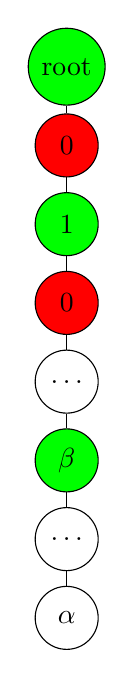
\begin{tikzpicture}[every node/.style={circle,draw,minimum size = 8 mm}]
  \node [fill = green](root) at (1,0) {root};
    \node [fill=red](zero) at (1,-1) {$0$};
    \node [fill=green](one) at (1, -2) {$1$};
    \node [fill=red](zero2) at (1,-3) {$0$};
    \node(dots) at (1,-4) {$\ldots$};
    \node[fill=green](beta) at (1,-5) {$\beta$};
    \node (dots2) at (1,-6) {$\ldots$};
    \node (alpha) at (1, -7) {$\alpha$};
    \draw (root) -- (zero);
    \draw (zero) -- (one);
    \draw (one) -- (zero2);
    \draw (zero2) -- (dots);
    \draw (dots) -- (beta);
    \draw (beta) -- (dots2);
    \draw (dots2) -- (alpha);
\end{tikzpicture}
    \caption{Legitimate alternating path}
    \label{fig:legitimate_alternating_path}
\end{subfigure}
\hfill
\begin{subfigure}[b]{0.3\textwidth}
\centering
    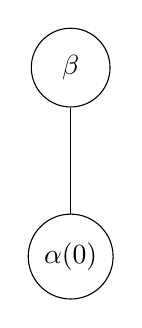
\begin{tikzpicture}[yscale=1.2,every node/.style={circle,draw,minimum size = 10 mm}]
  \node (b) at (1,0) {$\beta$};
    \node (a) at (1,-2) {$\alpha(0)$};
    \draw (b) -- (a);
\end{tikzpicture}
\quad
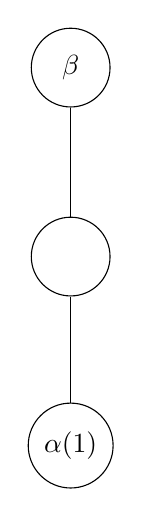
\begin{tikzpicture}[yscale=1.2,every node/.style={circle,draw,minimum size = 10 mm}]
  \node (b) at (1,0) {$\beta$};
  \node (c) at (1, -2) {};
    \node (a) at (1,-4) {$\alpha(1)$};
    \draw (c) -- (a);
    \draw (b) -- (c);
\end{tikzpicture}
    \caption{Parent or grandparent of $\alpha$ is $\beta$}
    \label{fig:parent_alpha}
\end{subfigure}
\hfill
\begin{subfigure}[b]{0.3\textwidth}
    \centering
    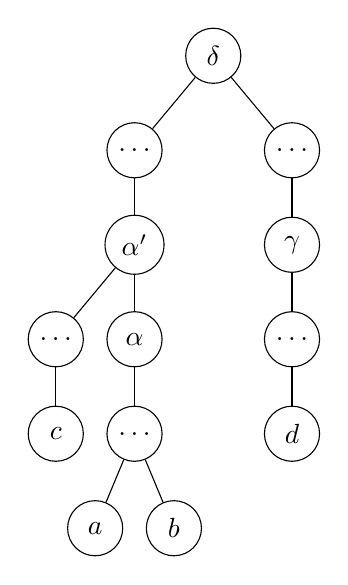
\begin{tikzpicture}[yscale=1.2,every node/.style={circle,draw,minimum size = 7 mm}]
  \node (b) at (1,0) {$\delta$};
    \node (a) at (0,-3) {$\alpha$};
    \node (pa) at (0, -2) {$\alpha'$};
    \node (e) at (0, -1) {$\ldots$};
    \node (e2) at (2, -1) {$\ldots$};
    \node (e3) at (-1, -3) {$\ldots$};
    \node (g) at (2, -2) {$\gamma$};
    \node (c) at (-1, -4) {$c$};
    \node (e4) at (0,-4) {$\ldots$};
    \node (reala) at (-0.5,-5) {$a$};
    \node (realb) at (0.5,-5) {$b$};
    \node (e5) at (2, -3) {$\ldots$};
    \node (d) at (2, -4) {$d$};
    \draw (g) -- (e5);
    \draw (e5) -- (d);
    \draw (e4) -- (realb);
    \draw (e4) -- (reala);
    \draw (a) -- (e4);
    \draw (e) -- (pa);
    \draw (b) -- (e);
    \draw (b) -- (e2);
    \draw (e2) -- (g);
    \draw (pa) -- (e3);
    \draw (e3) -- (c);
    \draw (a) -- (pa);
\end{tikzpicture}
    \caption{Proving existance of $P_4$ in condition $1$ of the theorem \ref{theorem_adding_equivalent}}
    \label{fig:theorem_1}
\end{subfigure}
\caption{Examples of cograph structure}
\end{figure}



\begin{theorem}[Theorem 1 \cite{corneil_perl_stewart_85}]
    \label{theorem_adding_equivalent}
     The given graph $G$ is a cograph if and only if none of the following conditions are true:
    
\begin{enumerate}
    \item there exists a $(0)$-node in $M \setminus \{\alpha\}$,
    \item there exists $v \in$ $ M \setminus \{\alpha\}$, such that $v$ is a $(1)$-node and is not properly marked,
    \item there exists $y \in M \setminus \{\alpha\}$, such that $y \neq R$ and the grandparent of $y \notin M \setminus \{\alpha\}$,
    \item The vertices of $ M \setminus \{\alpha\}$ do not lie on one path to $R$,
    \item $\alpha$ is a $(0)$-node whose parent is not $\beta$,
    \item $\alpha$ is a $(1)$-node which has a grandparent which is not $\beta$.
\end{enumerate}
\end{theorem}
It is easy to prove that this theorem is equivalent to the \Cref{theorem_adding}.

\subsection{Theorem \ref{theorem_adding_equivalent}}
Now let us prove that if condition $1$ of the Theorem \ref{theorem_adding_equivalent} is true, then $G$ is not a cograph. The other cases are similar.

From now on let $des (x)$ denote the leaves of the subtree of $x$, $\gamma$ be some $(0)$-node in $M \setminus \{\alpha\}$ and $\delta$ be the LCA of $\alpha$ and $\gamma$. 

We have to consider four cases, depending of what label do $\alpha$ and $\delta$ have. Here we consider their labels are both $0$ (see \Cref{fig:theorem_1}). The other cases follow similarly.

Let $\alpha'$ be the parent of $\alpha$. As it was said above, if all leaves in the subtree are the neighbours of $x$, then this node is ``marked-and-unmarked'', but we look at the nodes in $M$. Such nodes have at least one neighbour of $x$ and one not neighbour of $x$ in their subtrees. So, $a \in des(\alpha)$ is the neighbour of $x$,$b \in des(\alpha)$ is not a neighbour of $x$, $c \in des (\alpha') \setminus des(\alpha)$, $d \in des (\gamma)$ (except one case under) is the neighbour of $x$. If c is the neighbour of $x$, the $P_4$ is $b-c-x-d$, else $b-c-a-x$. But if $\delta = \gamma$,  $d \in des(y) \setminus des(\theta)$, where $\theta$ is the child of $\gamma$ on the $\alpha - \gamma$ path. 



\subsection{\texttt{FIND-LOWEST}}
Function \texttt{FIND-LOWEST} finds $\alpha$, the lowest marked node of cotree. 

\subsection{\texttt{ADD-VERTEX}}
Let us prove of one of many cases of the function \texttt{ADD-VERTEX} -- when $u$ is a $(0)$-node and the size of $A[0]$ does not equal to $1$. The other cases are similar. We use the notation from function \texttt{ADD-VERTEX} implementation. 
\begin{theorem}
    For each pair of leaves $(a,b)$ in the modified cotree $T'$, where $x \notin \{a, b\}$, the labels of LCA$_T(a,b)$ and LCA$_{T'}(a,b)$ are the same.
\end{theorem}
\begin{proof}
We call a vertex \emph{beautiful} if it is from the subtree of some vertex from $A[0]$ and \emph{ugly} if it is from the subtree of some child of $u$, such that $u$ is not in $A[0]$.

There are two states of every vertex -- is in the subtree of $u$, which in turn divided into beautiful and ugly, and is not in the subtree of $u$.
        \begin{itemize}
            \item if $a$ and $b$ are not from the subtree of $u$, then their LCA stays the same,
            \item If exactly one node (only $a$ or only $b$) is from the subtree of $u$ and the other is not from subtree of $u$, then their LCA is still the same,
            \item if $a$ and $b$ are both beautiful or both ugly, then if their LCA is not $u$, then it remains the same. If their LCA is $u$, then if $a$ and $b$ are beautiful, it becomes $y$, that has the same label as $u$; and if $a$ and $b$ are ugly, then their LCA is still $u$.
            \item if exactly one between $a$ and $b$ is beautiful and the other is ugly, then their LCA is still $u$.
        
        \end{itemize}
From the description of the algorithm, all vertices from $A[0]$, i.e. beautiful ones are now the children of $y$. Now we consider a beautiful node $l$ and an ugly node $r$ (see \Cref{fig:ADD-VERTEX}). $L(l)$ are all neighbours of $x$, because $l$ is ``marked-and-unmarked''. There are no neighbours of $x$ in $L(r)$, because $r$ is ``unmarked''.
\end{proof}
Now it's time to consider the case when $a=x$ or $b=x$. 
\begin{theorem}
    For every $b \neq x$ from $L(u)$, the label of the LCA of $x$ (the vertex that we are inserting to the cograph) and $b$, is correct.
\end{theorem}
\begin{proof}
Let us split the proof into the several cases:
        \begin{itemize}
            \item If $b$ is from $L(l)$ then their LCA is a new $(1)$-node and it is correct, because in $L(l)$ are only neigbours of $x$,
            \item If $b$ is from $L(r)$ then their LCA is $u$ and it is correct, because $u$ is $(0)$-node and in $L(r)$ there are no neighbours of $x$,
        \item If $b$ is not from $L(u)$, then we know that the path between $u$ and $R$ is a legitimate alternating path. 
        \begin{itemize}
            \item If the LCA of $x$ and $b$ is a $(0)$-node, and we know it is not marked, i.e. among its children there are not ``marked-and-unmarked'' vertices. Due to the existence of a legitimate alternating path we know than in the subtree of LCA,  excluding the subtree of its properly marked $(1)$-node, there are no ``marked'' vertices.  Therefore, every such child of LCA is ``unmarked'', and this logic can be recursively applied conclude that $L(LCA)$ has no neighbours of $x$, making it the correct LCA,
            \item If the LCA is a $(1)$-node, and we know it is properly marked, it has exactly one not ``marked-and-unmarked'' child, and this child is an ``unmarked'' $(0)$-node and the other children are ``marked-and-unmarked''. For every such child $c$ we know that $L(c)$ consists only of neighbours of $x$, making it the correct LCA too.
        \end{itemize}
        \end{itemize}
\end{proof}
        
\begin{figure}
    \centering
    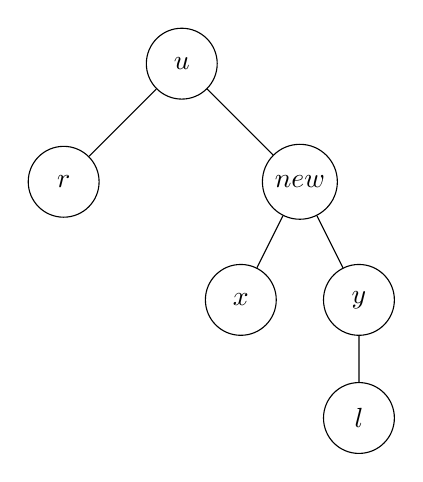
\begin{tikzpicture}[xscale=1.5,every node/.style={circle,draw,minimum size=9mm}]
  \node (u) at (1,0) {$u$};
  \node (l) at (2.5, -4.5) {$l$};
  \node (r) at (0, -1.5) {$r$};
  \node (new) at (2,-1.5) {$new$};
  \node (x) at (1.5,-3) {$x$};
  \node (y) at (2.5,-3) {$y$};

    \draw (y) -- (l);
    \draw (u) -- (r);
  \draw (u) -- (new);
  \draw (new) -- (x);
  \draw (new) -- (y);
\end{tikzpicture}
    \caption{\texttt{ADD-VERTEX} special case proof}
    \label{fig:ADD-VERTEX}
\end{figure}        

\section{Complexity}
\begin{theorem}
    Each iteration takes $O(\deg(x))$ time.
\end{theorem}
\begin{proof}
\texttt{MARK}: each node except root has a minimum of two children. If we imagine that all vertices, which are not neighbours of $x$ don't exist, then the tree has $\deg(x)$ leaves and the previous layer has at most $\frac{\deg(x)}{2}$ vertices, the one before that has at most $\frac{\deg(x)}{4}$ and so on. To calculate the total complexity we need to sum $\deg(x) + \frac{\deg(x)}{2} + \frac{\deg(x)}{4} + \dots$, which forms a geometric progression. The sum is at most $2 \cdot \deg(x)$, so it is $O(\deg(x))$. Therefore, the size of $M$ is also $O(\deg(x))$. For each node, processing time is $O(1)$, and the total time complexity of this function is $O(\deg(x))$.

\texttt{FIND-LOWEST}: each node from $M$ is processed in $O(1)$ time, the total complexity of this function is also $O(\deg(x))$.

\texttt{ADD-VERTEX}: all cases of inserting require $O(1)$ time, but the operation of removing elements of $A$ from $u$ to $y$ is $O(\deg(x))$, because $|A| \leq |M|$. 

\end{proof}
Therefore, the total time complexity of the algorithm is $O( \sum\limits_{v \in V}^{} \deg(v)) = O(n+m)$.

\chapter{A linear time cograph recognition algorithm of Bretscher, Corneil, Habib and Paul}
\section{Introduction}
Let us consider a linear recognition algorithm by Bretscher, Corneil, Habib and
Paul \cite{Bretscher2003ASL}.
The correctness of this algorithm may be difficult to understand, but the idea of the algorithm is quite easy. The hardest part of the linear implementation is to choose the right data structures. The coding part is long enough.
\section{Idea}
We choose an arbitrary permutation of our graph vertices. We define a LexBFS on it, then LexBFS-, which can be implemented using LexBFS. Finally, we define \texttt{Neighbourhood Subset Property} on a permutation. Having these definitions, our algorithm is short and simple:
\input{code/LexBFS-recognition}
\section{LexBFS}
\subsection{Idea}
We process vertices one by one and divide them into groups according to the property that the vertices in the same group have the same set of already processed neighbours. 
\subsection{Implementation}
Let us introduce the following notation: $N'(x) = \{v \colon v \in N(x)$ and $v$ has not been processed$\}$.

We only store groups consisting of unprocessed vertices. A list is maintained comprising these groups. Initially, the list contains only one group that includes all graph vertices. In each step we choose the leftmost group $A$, then choose the leftmost vertex $x$ in $A$. For every group $B$ we select all neighbours of $x$ in $B$, remove them from $B$ and place them in a new group $C$, which is inserted directly before $B$ in the list. Subsequently, we eliminate $x$ from $A$ and mark it as ``processed''. It is important to note that $B$ may be the same as $A$. Refer to the pseudocode in \Cref{pseudocode_lexbfs} and the example in the \Cref{tab:table} for further details.

\subsection{Pseudocode}
\label{pseudocode_lexbfs}
\input{code/LexBFS}
\begin{table}[H]
\centering
\begin{tabular}[,]{ | p{6mm} | p{3mm} | p{25mm} |  p{35mm} | }
\hline
 $\sigma(v)$ & $v$ & $N'(v)$ & Partitions \\ [0.5ex] 
 \hline\hline
 & & & $\{x$ $d$ $y$ $u$ $v$ $w$ $c$ $a$ $z$ $b\}$ \\
 \hline
 $1$ & $x$ & $\{u$ $v$ $w$ $y$ $z\}$ & $\{y$ $u$ $v$ $w$ $z\}$ $\{d$ $c$ $a$ $b\}$ \\
 \hline
 $2$ & $y$ & $\{a$ $b$ $c$ $d$ $w$ $z\}$ & $\{w$ $z\}$ $\{u$ $v\}$ $\{d$ $c$ $a$ $b\}$ \\
 \hline
 $3$ & $w$ & $\{a$ $b$ $c$ $d$ $z\}$ & $\{z\}$ $\{u$ $v\}$ $\{d$ $c$ $a$ $b\}$ \\
 \hline
 $4$ & $z$ & $\{a$ $u$ $v\}$ & $\{u$ $v\}$ $\{a\}$ $\{d$ $c$ $b\}$ \\
 \hline
 $5$ & $u$ & $\{a$ $b$ $c$ $d$ $v\}$ & $\{v\}$ $\{a\}$ $\{d$ $c$ $b\}$ \\
 \hline
 $6$ & $v$ & $\{a$ $b$ $c$ $d\}$ & $\{a\}$ $\{d$ $c$ $b\}$ \\
 \hline
 $7$ & $a$ & $\{\}$ & $\{d$ $c$ $b\}$ \\
 \hline
 $8$ & $d$ & $\{b$ $c\}$ & $\{c$ $b\}$ \\
 \hline
 $9$ & $c$ & $\{b\}$ & $\{b\}$ \\
 \hline
 $10$ & $b$ & $\{\}$ &  \\
 \hline
 \end{tabular}
 \caption{LexBFS example for the cograph $G$ from \Cref{fig:graph_example}}
    \label{tab:table}
 \end{table}
\section{LexBFS-}
\subsection{Idea}
LexBFS- is similar to LexBFS with one difference -- we specify further how we divide one group into two ones.
\begin{definition}[Definition 1 from \cite{Bretscher2003ASL}]
    The vertices in the leftmost partition of line $5$ of Algorithm LexBFS($G$, $V$) are tied when their neighbourhoods of processed vertices are
identical. We refer to such a set of tied vertices as a \emph{slice}, $S$.

When vertices from one slice are divided into two slices, we call it a \emph{tie breaking mechanism}.

The \emph{borders} of the slice $S$ are called two numbers $l$ and $r$, such that the set of vertices of $S$ is exactly the same as the set of vertices located at indexes between $l$ and $r$ in the answer permutation of LexBFS. 
\end{definition}
The tie breaking mechanism in LexBFS is very simple -- by taking the leftmost vertex of the slice. As for LexBFS-, it differs from LexBFS in the way it chooses the vertex from the slice -- it selects the leftmost vertex in the given permutation among all other vertices in the slice.

\subsection{Implementation}
Let us introduce the definitions that are required to understand this part of the algorithm.

\begin{definition}[Definition 2 from \cite{Bretscher2003ASL}]
    Let $S = [x, S^A(x), \langle S^N(x) \rangle]$ be an arbitrary slice constructed during a LexBFS sweep where $x$ is the first vertex of $S$. We consider only the first level of nested subslices of $S$. Let $S^A(x) = [$the subslice of $S$ of vertices adjacent to $x]$. Each subsequent subslice of $S$ contains vertices not adjacent to $x$. Let $\langle S^N(x)\rangle = (S^N_1(x), S^N_2(x), \ldots , S^N_k(x))$ denote the subslices not adjacent to $x$ in $S$.

    We similarly define $\overline{S} = [x, \overline{S^A(x)}, \overline{\langle S^N(x) \rangle]}$ with respect to the complement $\overline{G}$.
\end{definition}

For the previous example (see \Cref{fig:graph_example}), $S^A(x) = \{y, u, v, w, z\}$, $S^N_1(x) = \{a\}$, $S^N_2(x) = \{d, c, b\}$. If initial ordering is $x y u w z a d c b$, then the slices for the $\overline{G}$ are $x[dacb][z][uwyv]$.

It is worth to say that when we write $S^A(x)$ and $\langle S^N(x) \rangle$, it does not mean that we start LexBFS from the beginning with $x$ as a first vertex -- but we do it inside its slice. With fixed initial permutation the total size of $S^A(x)$ and $\langle S^N(x) \rangle$ is the size of the slice of $x$ minus 1. For the first element of permutation, this sum is equal to $n-1$.

The example of nested slices for vertex $y$ for LexBFS of $G$ is $x[y[wz][uv]][a][dcb]$, so $S^A(y)=[wz]$ and $S^N_1(y)=[uv]$. For vertices $y$ and $a$ for LexBFS of $\overline{G}$ is $x[a[d[][cb]]][z][y][y[uv][w]]$, so $S^A(y)=[uv]$ and $S^N_1(y)=[w]$.

\subsubsection{Implementation and complexity}
The optimal implementation LexBFS- on $G$ runs in $O(n+m)$ time, that is, if we implement $L$ as a list of lists, representing the groups of unprocessed vertices. For each vertex, we can maintain a pointer to a list(a group) it belongs to. Removing the neighbours of $x$ from some group $A$ can be done in $O(\deg(x))$ time. This is achieved by examining the pointer to the group of each unprocessed neighbor $y$ and removing $y$ from $A$. If $y$ is the first element removed from $A$ during the iteration of the algorithm, a new list containing only $y$ is created and placed before $A$ in $L$. If $y$ is not the first element removed from $A$, it is inserted into the list before $A$ in $L$. This operation takes $O(1)$ time for each $y$.

While processing vertex $x$ we store the number of vertices in $S^A(x)$ and the total capacity of $S^N_i(x)$, which indicate the number of neighbours and not neighbours of its slice respectively. With this information, for every index $i$ we know for each vertex $y$ if $i$ is the end of $S^A(y)$. The list of such vertices is denoted as $D$. For each $z$ in $D$ we know that at this moment the neighbours of $z$, i.e. $S^A(z)$ are processed. This implies that the non-neighbours of $z$ have already been partitioned into the slices now. Therefore, we know $S^N_j(z)$ for every $j$, enabling us to outline the borders of each $S^N_j(y)$ in an array, which proves beneficial in the subsequent function.

\section{Neighbourhood Subset Property}
To understand this property we need to introduce it first formally via the following definitions:

\begin{definition}[Definition 4 from \cite{Bretscher2003ASL}]
    Given a slice $S^N_i(v)$ we define the \emph{processed neighbourhood} of $S^N_i(v)$ to be
$N_i(v) = \{y \colon y$ is processed and for every $z$ from $S^N_i(v)$ holds $y \in N(z)\}$.
\end{definition}

\begin{definition}[Definition 5 from \cite{Bretscher2003ASL}]
    LexBFS satisfies the \emph{Neighbourhood Subset Property} if and only if $N_{i+1}(v) \subseteq N_i(v)$, for all $v \in V$ and for all $i \geq 1$.
\end{definition}
Before we elaborate on the meaning of this property (see \Cref{correctness_lexbfs}), let us proceed with its implementation details.
\subsection{Implementation}
We use the following notation: let $c$ be the resulting ordering from the second LexBFS pass in the algorithm and $d$ be the resulting ordering from the third LexBFS pass in the algorithm.


For every $x$ and $i$ we know the borders of $S^N_i(x)$ in $c$ and $\overline{S^N_i(x)}$ in $d$. Therefore, for each $x$ we can compare the set of processed neighbours of first vertices $a$ and $b$ of $S^N_i(x)$ and $S^N_{i+1}(x)$ respectively. We can check only the first vertices in these slices because due to the definition of a slice, all vertices in it have the same set of processed vertices.

For every vertex $v$ let us define $used[v]=1$ if $v$ is a neighbour of $a$ in $G$, and $used[v]=0$ otherwise. And for every neighbour $w$ of $b$ we just need to verify if $used[w] = 1$.

When we do it for the complement of the graph and the result permutation $d$, the procedure is similar. We need every processed neighbour of $\overline{S^N_i(x)}$ to be a neighbour of $\overline{S^N_{i+1}(x)}$, because a neighbour in $G$ is not a neighbour in $\overline{G}$.
Additionally, we need to separately verify that $\overline{S^N_{i+1}(x)}$ does not contain any element of $\overline{S^N_i(x)}$ as a neighbour.

\section{Cotree}
\subsection{Idea}
The wonderful fact is if we start building a cotree with some vertex $x$, then we just need to build a path of $(0)$-nodes and $(1)$-nodes and cotree for slice $S^N_i(x)$ corresponds to the $i^{th}$ $(0)$-node and the cotree for slice $\overline{S^N_i(x)}$ corresponds to the 
$i^{th}$ $(1)$-node. Thus, we can just build these parts of the cotree recursively, using the fact, that we already know every $S^N_i(x)$ and $\overline{S^N_i(x)}$ recursively. 
\subsection{Implementation}
\input{code/cotree_LexBFS}
\section{Complexity}
\subsection{LexBFS and LexBFS-}
LexBFS on $\overline{G}$ also runs in $O(n+m)$ time, because in the line 10 of LexBFS implementation on $G$ (see \Cref{pseudocode_lexbfs}) we can just move $q$ to the right of $g$. Although there are the neighbours of $x$ in the graph $G$ within the group $g$, then there are no neighbours of $x$ in $\overline{G}$ within the group $g$. Similarly, there are only neighbours of $x$ in $\overline{G}$ within $q$. So when we insert $g$ not to the left of $q$, but to the right, then their order now is $(q, g)$ and in $q$ there are no neighbours of $x$ in $\overline{G}$, while in $g$ there are only neighbours of $x$ in $\overline{G}$. Thus, the list was partitioned into two lists: the left list are neighbours and the right one are not the neighbours. This is what we wanted to show.

LexBFS- on $G$ can also be implemented in $O(n+m)$ time. We achieve this by making the initial permutation equal to the given parameter permutation $\pi$ and running the usual LexBFS algorithm. So when we select the leftmost element, it is processed earliest with respect to other elements in its slice. This behavior arises because the initial permutation is $\pi$ and the elements inside the slice do not change places relative to each other. Our only modification involves removing some vertices from the slice in the same order and inserting them into a new slice. 
\subsection{Neighbourhood Subset Property}
Let us denote by $NS(S)$ the number of all non-empty $S^N_i(x)$ for every $i$ and $x$ for some slice $S$.
\begin{theorem}
    $NS(S) \le |S| - 1$.
\end{theorem}
\begin{proof}
    It can be proved by induction. The base case for $n=1$ holds since $NS(S)=0$. In the induction step we know that
    for every $i$ $NS(S^N_i(x))$ by induction is no more than $|S^N_i(x)| - 1$. Therefore, if $m$ is the number of non-empty slices $S^N_i(x)$, then:
    \begin{align*}
        NS(S) = m + \sum_{i=1}^{m} NS(S^N_i(x)) \le m + \sum_{i=1}^{m} (|S^N_i(x)| - 1) =  m + \sum_{i=1}^{m} |S^N_i(x)| - m \\
        = \sum_{i=1}^{m} |S^N_i(x)| \le |S| - 1
    \end{align*}
    The last inequality is in fact equality if and only if $x$ has no neighbours in $S$.
\end{proof}

\begin{theorem}
    For every vertex $v$ it is the first vertex for no more than one $S^N_i(x)$ for some $x$ and $i$.
\end{theorem}
\begin{proof}
    Let us consider the slice $S^N_i(x)$ with the largest size, in which $v$ is the first vertex. $S^N_i(x)$ is recursively divided into $v$, $S^A(v)$ and $\langle S^N(v) \rangle$, but $v$ cannot be the first vertex of $S^N_i(v)$ for any $i$. And we know that $S^N_i(x)$ is the largest slice, so $S^N_i(v)$ for some $i$ is the only option to $v$ to be the first vertex in the slice.
\end{proof}

Due to the previous theorems, we can build an injective mapping between the set of non-empty slices and the set of vertices. All representatives, i.e. first vertices of slices, are unique, so the sum of their degrees is no more than $2 \cdot m$.

Therefore, we can just iterate through every existing non-empty slice $S^N_i(x)$ and check if its neighbourhood of processed vertices is a superset of $S^N_{i+1}(x)$, if it exists. As mentioned above, we have at most $n-1$ such non-empty slices $S^N_i(x)$ for every $x$ and $i$ and the first vertex of each slice is unique. Consequently, they have no more than $2 \cdot m$ neighbours in total. Let $v$ be the first vertex of $S^N_i(x)$ and $w$ be the first vertex of $S^N_{i+1}(x)$. Comparing the sets of processed neighbours of $v$ and $w$ takes $O(\deg(v) + \deg(w))$ time. Therefore, the total time complexity is $O(n+m)$ time. 
\section{Correctness}
\label{correctness_lexbfs}
The idea of the proof is based on the fact, that there is a bijection between cographs and cotrees. Therefore, if a valid cotree exists for this graph, then this graph is a cograph. 

We need to understand when we can build a cotree from the slice sequences. Slices $S^N_i(x)$ corresponds to sub-cotrees, as mentioned in the Cotree section. The processed neighbours of $S^N_{i+1}(x)$ form a subset of processed neighbours of $S^N_i(x)$. Equivalently, the processed neighbours of vertices of $(i+1)^{th}$ $(0)$-node subtree, are a subset of the processed neighbors of vertices in the $i^{th}$ $(0)$-node subtree. Consider any vertex $z$ from $S^N_{i+1}(x)$. If some $y$ is a processed neighbour of $z$, then their LCA is $(1)$-node due to the cotree property. But some vertex $t$ from $S^N_i(x)$ is in the subtree of the $i^{th}$ $(0)$-node, i.e. in the subtree of grandchild of the $(i+1)^{th}$ $(0)$-node. This implies that LCA$(t,y) = $ LCA $(y,z)$. Therefore, it is $(1)$-node. 

Furthermore, LCA of a vertex from $S^N_i(x)$ and a vertex from $S^N_{i+1}(x)$, is the $(i+1)^{th}$ $(0)$-node. Consequently, they can not be neighbours if this graph is a cograph.

In summary, the statement ``a valid cotree exists if the neighbourhood subset property is true for both results permutations'' aligns with the reasoning presented above. 

Similar reasoning also holds also for $\overline{G}$ and its corresponding slices, i.e. $\overline{S^N_i(x)}$ instead of $S^N_i(x)$.

\chapter{A $O((m + n) \cdot \log{n})$ time cograph recognition algorithm of Dahlhaus}
\section{Introduction}
Let us consider a parallel recognition algorithm in $O(\log^2{n})$ time and 
$O(n + m)$ processors by Dahlhaus \cite{dahlhaus_95}. 
We will consider the sequential version of this algorithm in $O((m + n) \cdot \log{n})$ time.
This algorithm is easier than the previous ones, but it has a big constant hidden in the asymptotic notation, because of many operations performed in every iteration.

\section{Idea}
We proceed with finding the cotree for our graph by dividing the graph into groups of induced subgraphs and recursively computing cotrees on them and merging them into one cotree. Once we have the cotree, we can determine whether the graph is a cograph. Let us assume the cotree $T$ that we have found corresponds to $G'=(V, E')$. Our goal is to check that $E = E'$. To check this we perform two actions:
\begin{itemize}
    \item for every connected pair of vertices $\{x$,$y\} \in E$ in our graph we check that LCA$(x,y)$ in the cotree is a $(1)$-node,
    \item for every $(1)$-node $z$ in the cotree, we compute the number of pairs of leaves $x$, $y$, such that LCA$(x,y) = z$. It is equivalent to getting the number of edges in the graph corresponding to the cotree.
\end{itemize}

Suppose that there exists a vertex $v$ such that $\frac{n}{a} \leq \deg{v} \leq \frac{n(a - 1)} {a}$. The case when such vertex does not exists considered in the \Cref{high_and_low}. Next, we divide the remaining vertices into two induced subgraphs -- $A$, which consists of the neighbours of $v$, and $B$, which consists of non-neighbours of $v$. Then we partition $B$ into connected components, i.e. induced subgraphs $B_0$, $B_1$, $\ldots$, $B_k$, and reorder them according to some rules. After that, by using this reordered partitioning we divide $A$ into induced subgraphs $A_0$, $A_1$, $\ldots$, $A_{k+1}$. Finally, we recursively compute the cotrees for every $A_i$ and $B_i$ and connect them. We do it by connecting the root of the cotree of $B_i$ to the $i^{th}$ $(0)$-node and connect the root of the cotree of $A_i$ to the $i^{th} (1)$-node (see \Cref{fig:cotree_build}).

\begin{figure}
    \centering
    \begin{tikzpicture}[xscale=1.4,yscale=0.85,every node/.style={circle,draw,minimum size=13mm},level distance=2cm,
  level 1/.style={sibling distance=4cm},
  level 2/.style={sibling distance=2cm},
  level 3/.style={sibling distance=2cm},
  level 4/.style={sibling distance=2cm}]
    
    \node {$1$}
        child { node {$0$}
            child { node {$T_{A_k+1}$}
            }
        }
        child { node {$0$}
        child { node {$T_{B_k}$}
            }
            child{ node{$\ldots$}
                child{ node{$0$}
                    child{node{$T_{B_0}$}}
                    child{ node{$1$}
                        child{node {$0$} child{node {$T_{A_0}$}}}
                        child{node{$v$}}
                    }
                }
            } 
        };
\end{tikzpicture}
    \caption{Cotree building procedure}
    \label{fig:cotree_build}
\end{figure}


\begin{minted}[
frame=lines,
framesep=2mm,
baselinestretch=1.2,
fontsize=\footnotesize,
linenos
]{c++}
add(type t, graph H) {
  x = new (t)-node;
  x.add_child(T.root);
  T.root = x;
  if (t == 0) {
    x.add_child(build_cotree(H).root);
  } else {
    y = new (0)-node;
    x.add_child(y);
    y.add_child(build_cotree(H).root);
  }
}

build_cotree(G) {
  v = arbitrary chosen vertex from G;
  compute B[0], .., B[k];
  reorder B[0], .., B[k];
  compute A[0], .., A[k + 1];
  create empty cotree T;
  T.root = v;
  for (i in [0..k+1]) {
    add(1, A[i]);
    if (i == k + 1) {
      break;
    }
    add(0, B[i]);
  }
}
\end{minted}

\section{Implementation}
Now all that remains is to understand how to reorder $\{B_i\}$ and compute $\{A_i\}$.
\subsection{Reordering $B_i$}
\begin{definition}
    For a set $W \subseteq V$, we denote by \emph{$\Gamma(W)$} $=$ $\{v \in V \setminus W \colon$ there exists $w \in W$ such that $\{v,w\} \in E\}$ the set of neighbours of W which are not in W.
\end{definition}
  

When we compute $B_i$, let us take one element $x \in B_i$. For $x$ we compute the set $C_i = \{v \colon v \notin B_i $ and $\{x,v\} \in E \}$. Later we will show that $C_i=\Gamma{(B_i)}$. It is sufficient to sort the set $\{B_i\}$ by the size of $\{C_i\}$ in descending order using bucket sort.
\subsection{Computing $A_i$}
\label{compute_a}
Next, for all $i = 0,1,\ldots,k-1$ we compute $C_i \setminus C_{i+1}$. The induced subgraph $A_{i+1}$ is formed by the vertices in $C_i \setminus C_{i+1}$. Similarly, $A_0$ is induced by $V \setminus (\{v\} \cup C_0)$ and $A_{k+1}$ is induced by $C_{k}$.
The effective implementation requires to find the largest $j$, such that element $y$ appears in $C_j$, then $y \in A_{j+1}$. If $y$ does not appear in any $C_j$, then we know that $y \in A_0$.
\subsection{Checking the correctness of the cotree}
The algorithm for finding LCA in $O(\log{n})$ time for query and $O(n \cdot \log{n})$ pre-calculation time, where $n$ is the size of the tree is well-known, so it will not be discussed here. The curious reader can be referred to \cite{LCA}.

Let us find, for every $(1)$-node $z$ the number of leaves $x, y$, such that LCA$(x,y)=z$. Assume that $z$ has $p$ children denoted by $z_0,\ldots,z_{p-1}$. For every $i$ it holds that LCA of two leaves from subtree rooted in $z_i$ is different from $z$. But LCA$(x,y)=z$, for every $x, y$ where $x$ is a leaf from $z_i$ and $y$ is a leaf from $z_j$ with $i \neq j$. Therefore, we just need to calculate the number of such pairs.

\begin{definition}
    For every vertex $q$, let us denote by \emph{$leaves[q]$} the number of leaves in subtree of $q$.
\end{definition}

It is easy to spot that for every $q$ $leaves[q]$ can be calculated using well-known techniques of dynamic programming and depth first search, so we skip its details. Let us instead continue with the main algorithm. To get the number of pairs $x,y$, such that LCA$(x,y)=z$ we initialize a variable $sum$ by zero. Then, for every $i=0,\ldots,p-1$ we just multiply $leaves[z_i]$ by  $\sum_{j \neq i}^{}leaves[z_j]$ and add this value to $sum$. Finally, we divide the $sum$ by $2$, because each pair was counted twice.  
\section{Complexity}
Computing the connected components, i.e. $\{B_i\}$ can be done in $O(n+m)$ time. Counting $\{C_i\}$ also can be done in $O(n+m)$ time, because $\sum_{v \in V}^{} \deg(v) = 2 \cdot m$. The maximum size of $C_i$ is $n$, so bucket sort takes $O(n)$ time. The effective implementation of finding $\{A_i\}$ in \Cref{compute_a} can be done in $O(n+m)$ time, because  $O(\sum_{i=0}^{i=k} |C_i|) = O(n+m)$ and we can iterate through the elements of every $C_j$ just updating the maximum index position where element the element appears.

Furthermore, it holds that $A_i, B_i \leq \frac{n(a-1)}{a}$. Therefore, we divide the main problem into smaller ones and such small problems have sizes at most $\frac{n}{c}$ for some $c > 1$. As mentioned earlier, computing $\{A_i\}$, $\{B_i\}$ and $\{C_i\}$ is $O(n+m)$ time. Therefore, we can say that processing of each vertex and each edges takes $O(1)$. But one vertex or edge can be in at most $O(\log{n})$ problems, because if the last segment where it was has size $x$, then the previous one has size at least $xc$, the previous one has size at least $xc^2$, etc. The last one has size $n$.

Checking the cotree consists of counting array $leaves$ and $m$ queries. Counting array $leaves$ can be computed in $O(n+m)$ time, because we run one depth first search and pre-calculation is $O(n \cdot \log{n})$ time. We have $m$ edges, so we have $m$ queries and each query is $O(\log{n})$. So, checking the cotree runs in $O((m + n) \cdot \log{n})$ time. Therefore, the total time complexity of the algorithm is $O((m + n) \cdot \log{n})$.
\section{Correctness}
For every pair of vertices we need to show that if $G$ is a cograph, then their LCA label is correct.

None of the vertices of $B_i$ for every $i$ are connected with $v$, so it is correct to connect the cotree to $(0)$-node, because the LCA of $v$ and every vertex of $B_i$ is this $(0)$-node. The same also holds for $A_i$ and $(1)$-node.

The LCA of $x \in B_i$ and $y \in B_j$ is the $\max{\{i,j\}}^{th}$ $(0)$-node. This is correct because $B_i$ and $B_j$ are the connected components of $B$, so they do not have any edges between each other.

Since we build the cotrees recursively, so the LCA of a pair of leaves in each recursively computed cotree is correct. 

Therefore, it remains to show only that if $G$ is a cograph, then the LCA of $x \in A_i$ and $y \in A_j$ is correct and the LCA of $x \in B_i$ and $y \in A_j$ is correct too.

\begin{theorem}
\label{one_label_subtree}
    For every $i,j$ such that $0 \leq i < j \leq k + 1$ and every $x \in A_i$ and every $y \in A_j$ it holds that $\{x,y\} \in E$. 
\end{theorem}
\begin{proof}
    If for some $i,j$ such that $0 \leq i < j \leq k + 1$ there exists $x \in A_i$ and $y \in A_j$ and $\{x,y\} \notin E$, then for every $z \in B_{i-1}$ and for every $t \in B_{j-1}$ holds $\{z,x\}, \{y,t\}, \{z, y\} \in E$ and $\{x,t\} \notin E$, due to the definition of $\{A_i\}$ and $\{z,t\} \notin E$ due to the definition of $\{B_i\}$. Therefore, $x-z-y-t$ is $P_4$, the contradiction. Therefore, $\{x,y\} \in E$.
\end{proof}
Thus, the LCA of $x \in A_i$ and $y \in A_j$ where $i < j$, is correct, because it is exactly the $j^{th}$ $(1)$-node.

Therefore, it remains to show only that if $G$ is a cograph, then the LCA of $x \in B_i$ and $y \in A_j$ is correct too. To prove it we need to introduce the following definition and theorems.
\begin{definition}
    For every $i$ and for every $x \in B$ let us denote by \emph{$NB(B,x)$} the set of neighbours of $x$, which are not in $B$.
\end{definition}

\begin{theorem}
    For every $i$ and for every $x, y \in B_i$ it holds that $NB(B_i,x) = NB(B_i,y) = \Gamma{(B_i)}$
\end{theorem}
\begin{proof}
    If for some $i, j$ there exist $x \in B_i$ and $y \in B_i$ and $z \in A_j$, such that $\{x, z\}, \{x, y\} \in E$ and $\{y, z\} \notin E$, i.e. there exists a vertex where adjacent vertices $x$ and $y$ are not agreed. Then there exists $P_4 = v-z-x-y$, so $G$ is not a cograph. Therefore, for every $i$ and every pair of $x$ and $y$ from $B_i$, such that ${x,y} \in E$, has the same neighbourhood among the neighbours of $v$. And there do not exist $i \neq j$, $a$ from $B_i$ and $b$ from $B_j$, such that $\{a,b\} \in E$. So, $NB(B_i,x) = NB(B_i,y)$ if $\{x,y\} \in E$ and $x,y$ are from $B_i$. This implies that $NB(B_i,x) = NB(B_i,y) = \Gamma{(B_i)}$ for every pair $x,y$ from $B_i$, because $B_i$ is connected. 
\end{proof}
So, it is correct to look for the neighbours of only one vertex from $B_i$.

\begin{theorem}
    For $0 \leq i < j \leq k$ it holds that either $\Gamma{(B_i)} \subseteq \Gamma{(B_j)}$ or $\Gamma{(B_j)} \subseteq \Gamma{(B_i)}$, if $G$ is a cograph.
\end{theorem}
\begin{proof}
Assume it is not true, then for $x \in B_i$ and $y \in B_j$ there exist $z, t$, such that $\{x,z\},\{y,t\} \in E$ and $\{x,t\}, \{y,z\} \notin E$, but $\{x,y\} \notin E$ and $\{z,t\} \in E$, as mentioned earlier. Consequently, $x-z-t-y$ is $P_4$ in $G$, the contradiction.
\end{proof}

\begin{theorem}
\label{different_labels_subtree}
    For every $i,j$ and every $x \in A_i$, $y \in B_j$ it holds that $\{x,y\} \in E$ and LCA$(x,y)$ is $(1)$-node if and only if $j \geq i$.
\end{theorem}
\begin{proof}
    For every $i=0,\ldots,k+1$, every $x \in A_i$, every $j=i,\ldots,k$ and every $y$ in $B_j$, $\{x,y\} \notin E$ due to the definition of $A_i$. So, the LCA$(x,y)$ is correct, because the $i^{th}$ $(0)$-node, to which the cotree of $A_i$ is connected is lower than the $j^{th}$ $(1)$-node, to which the cotree of $B_j$ is connected, so their LCA is the $j^{th}$ $(1)$-node. The same argument also holds for every $j=0,\ldots,i-1$.
\end{proof}
\section{High and low vertices}
\label{high_and_low}
\begin{definition}
    A vertex $v$ is \emph{high} if its degree is greater than $\frac{n(a-1)}{a}$. A vertex $v$ is \emph{low} if its degree is smaller than $\frac{n}{a}$.
\end{definition}
We do not have a vertex in $G$ which degree is in the range $[\frac{n}{a}, \frac{n(a-1)}{a}]$, so now all vertices are high or low. Let us define by $L$ the set of all low vertices. It can be proved similarly to the previous case that every component of $L$ forms its subtree and that parents of these subtrees are on one path to root.

Similar to the previous case, we calculate $\Gamma(C_i)$ for each component $C_i$ of $L$, sort the components by the size of $\Gamma(C_i)$ and compute $D_i = \Gamma(C_i) \setminus \Gamma(C_{i+1})$. The only difference is that if for some $j$, $|D_j| > \frac{n(a-1)}{a}$, we run another algorithm. We know that there exists at most one such $j$. Let $H$ be the subgraph induced by $D_j$ . If in $\overline{H}$ there exists a non-high and non-low vertex, then we do not need to change anything, because when the recursion is called on $H$, it is divided into problems at least $\frac{a}{a-1}$ times smaller. If not, then there are only low vertices in $\overline{H}$, because in $D_j$ there only high vertices and in $\overline{H}$ there are no non-high and non-low vertices, so they are all low. So, we can build for each component of $\overline{H}$ a cotree and reverse it, so we can get a cotree for $H$.

\subsection{Correctness}
Similar to the previous case, we need to show, that the label of LCA of every pair of vertices is correct.
\begin{theorem}
    For every $i$,$j$ such that $0 \leq i < j \leq k$, every $x \in C_i$ and every $y \in C_j$ it holds that $\{x,y\} \notin E$. 
\end{theorem}
\begin{proof}
    $C_i$ and $C_j$ are disjoint connected components of $L$, so $x$ and $y$ cannot be connected.
\end{proof}


\begin{theorem}
    For every $i$,$j$ such that $0 \leq i < j \leq k + 1$, every $x \in D_i$ and every $y \in D_j$ it holds that $\{x,y\} \notin E$. 
\end{theorem}
\begin{proof}
    The proof is exactly the same as in the \Cref{one_label_subtree}.
\end{proof}

\begin{theorem}
    For every $i$ and every $\{a, b\} \in D_i$ such that $\{a,b\} \in E$, $NB(D_i,a)=NB(D_i,b)$. 
\end{theorem}
\begin{proof}
     Assume, to the contrary, that there exists a vertex $z \in D_j$ for some $j$, such that $\{a,z\} \in E$ and $\{b,z\} \notin E$. 
     
     There also exists a vertex $t$, such that $\{t,z\} \in E$ and $\{t,a\}, \{t,b\} \notin E$. If it is not true, than for every $t$ either $\{t,z\} \notin E$, or $\{t,a\} \in E$ or $ \{t,b\} \in E$. We know that $z$ is high, so the number of non-neighbours of it is not greater than $\frac{n}{a}$. Since $a, b$ are low, the number of their neighbours does not exceed $\frac{n}{a}$. Therefore, there are at least $\frac{n(a-3)}{a}$ vertices not meeting any of these criteria, i.e. at least $\frac{n(a-3)}{a}$ vertices $t$ such that $\{t,z\} \in E$, and $\{t,a\} \notin E$ and $ \{t,b\} \notin E$.

     Thus, there is an induced $P_4$ $b-a-z-t$ -- a contradiction.
\end{proof}


\begin{theorem}
    For every $i$,$j$ such that $0 \leq i < j \leq k + 1$ and every $x \in C_i$ and $y \in D_j$ it holds that $\{x,y\} \notin E$. 
\end{theorem}
\begin{proof}
    The proof is exactly the same as in the \Cref{different_labels_subtree}.
\end{proof}

\begin{theorem}
    For every $i$,$j$ such that $0 \leq i < j \leq k$ and every $x \in D_i$ and $y \in C_j$ it holds that $\{x,y\} \notin E$. 
\end{theorem}
\begin{proof}
    The proof is exactly the same as in the \Cref{different_labels_subtree}.
\end{proof}

\subsection{Complexity}
\begin{theorem}[Lemma 6 from \cite{dahlhaus_95}]
    Every connected component in the graph induced by low vertices has at most $\leq \frac{2n}{a} + 1$ vertices.
\end{theorem}
\begin{proof}
    Let $t$ be LCA of all vertices from $C_i$ for some $i$. Clearly, $t$ is $(1)$-node, because $C_i$ is connected. Assume $t$ has $k$ children denoted as $t_1,..., t_k$. We know that $k \geq 2$, because $C_i$ is connected. For some descendant leaf $v \in V$ of $t_1$, it must be connected with all $u \in V$, which are descendant leaves of $t_2,..., t_k$, because the label of their LCA is $1$. But $v$ is low, so its degree is at most $\frac{n}{a}$, so there are no more than $\frac{n}{a}$ vertices in $V$ among descendant leaves of $t_2, ..., t_k$. We do the same for $t_2$, so the total amount of vertices in the subtree of $t$, i.e. in $C_i$, does not exceed $\frac{2n}{a} + 1$.
\end{proof}

\begin{theorem}
    $\overline{H}$ can be computed in $O(n+m)$ time.
\end{theorem}
\begin{proof}
$H$ is a set of high vertices, because components of low vertices have sizes at most $\frac{2n}{a} + 1$.
    In $\overline{H}$ the degree of each vertex is at most $\frac{n}{a}$, because its degree in $G$ is at least $\frac{n(a-1)}{a}$. So, the total number of edges in $\overline{H}$ is bounded from above by $ \frac{n \cdot |H|}{a} \leq \frac{(a-2)n \cdot |H|}{a}$. On the other hand, $|H| \geq \frac{(a-1)n}{a}$, so the cardinality of $G \setminus H$ is bounded by $ \frac{n}{a}$, but every $v \in H$ has at least $\frac{(a-1)n}{a} - \frac{n}{a} = \frac{(a-2)n}{a}$ neighbours in $H$, so the number of edges in $H$ is at least $\frac{(a-2)n \cdot |H|}{a}$.

    
    Therefore, $H$ contains more edges than $\overline{H}$ and it contains at least half of the pairs from $\frac{|H|(|H|-1)}{2}$. So, we can iterate through every pair of vertex and check if they are connected, and they are not connected we add this edge to the complement of graph.
\end{proof}
So, like in the previous case, the problem is divided into the smaller ones with sizes at most $\frac{n}{c}$ for some constant $c > 1$. The time complexity remains the same as in the previous case, i.e. it is equal to $O((n+m) \cdot \log{n})$.
\chapter{Experiments}
All discussed algorithms and the other cograph recognition algorithm \cite{Habib2005ASL} were implemented and added to the Koala-NetworKit library \cite{Tur+23}. They were implemented in C++ using the NetworKit \cite{NKT+23} library and
the Koala \cite{Tur+23} library. 

\section{Implementation details}
Let us show the file structure. 

\textbf{CoTree files:}
\begin{itemize}
    \item \texttt{include/recognition/CoTree.hpp} -- header file, which defines cotree interface
    \item \texttt{cpp/recognition/cograph/CoTree.cpp} -- implementation of cotree interface
\end{itemize}
\textbf{Cograph recognition algorithm files:}
\begin{itemize}
    \item \texttt{include/recognition/CographRecognition.hpp} -- main header file, which defines default cograph recognition and other algorithm interfaces.
    \item \texttt{cpp/recognition/CographRecognition.cpp} -- implementation of default cograph recognition algorithms' interfaces.
    \item \texttt{cpp/recognition/cograph/CorneilStewartPerlCographRecognition.cpp} -- Corneil, Perl and Stewart algorithm implementation.
\item \texttt{cpp/recognition/cograph/BretscherCorneilHabibPaulCographRecognition.cpp} -- Bretscher, Corneil, Habib, Paul algorithm implemenation.
\item \texttt{cpp/recognition/cograph/DahlhausCographRecognition.cpp} -- Dahlhaus algoritm implementation.
\item \texttt{benchmark/benchmarkCographs.cpp} -- benchmarking programs to evaluate the correctness of every algorithm on different graphs.
\item \texttt{test/testCographRecognition.cpp} -- unit tests for evaluating the correctness of every algorithm.
\end{itemize}


\section{Benchmarking and performance evaluation}
Our benchmarking suite allows for a robust assessment of algorithm correctness and performance, testing on randomly generated graphs, as well as on all known fixed-size graphs and cographs and comparing the results.

The performance of the algorithms was thoroughly evaluated across a wide range of graph instances. By testing graphs of varying sizes and densities, we assessed the efficiency of each algorithm in different scenarios.  \Cref{tab:algorithms_number} displays the identifier assigned to each algorithm in the tables below.

We choose four random graph models for performance testing:
\begin{itemize}
    \item Erd\H{o}s-Renyi model --  it provides a wide variety of graph structures, ensuring comprehensive testing across different configurations of node connections. It is a standard model for testing graph algorithms,
    \item Barab\'asi-Albert model -- it produces a network with a few vertices of high degree and many vertices of low degree. If we initiate our algorithm with vertices of low degree, the algorithm can terminate much sooner than if we start with vertices of high degree. For instance, $A1$ is iterative and its performance is significantly influenced by the degrees of the processed vertices. So, this test allows us to obtain the ``best case'' scenario.
    \item Watts-Strogatz model -- all vertex degrees are identical and all paths are short, providing a more useful test than the previous one, allowing us to obtain the ``average'' scenario.
    \item Randomly generated cographs -- unlike graphs that are not cographs, the execution of the algorithms on a cograph cannot end earlier with a result ``not a cograph''. Therefore, this test allows us to maintain the ``worst-case'' scenario. 
\end{itemize}

All restrictions follow from the capabilities of the algorithms or the capabilities of the generator functions, some of which end with a SIGKILL error or hang due to large input data. Generators work longer than all algorithms. For each data set, only one graph was tested, since generating such large data is very time-consuming.
\begin{center}
\begin{table}[]
    \centering
    \begin{tabular}{ | c | p{10cm} |}
  \hline
  Number & Algorithm \\ [0.5ex] 
  \hline\hline
  $A1$ & A linear recognition algorithm for cographs by Corneil, Perl, Stewart \cite{corneil_perl_stewart_85} \\
  \hline
  $A2$ & A simple Linear Time LexBFS Cograph Recognition Algorithm by Bretscher, Corneil, Habib, Paul \cite{Bretscher2003ASL}\\
  \hline
  $A3$ & Efficient parallel recognition algorithms of and distance hereditary graphs by Dahlhaus \cite{dahlhaus_95}\\
  \hline
  $A4$ & A simple linear time algorithm for cograph recognition by Habib, Paul \cite{Habib2005ASL}\\
  \hline
  \end{tabular}
  \caption{The algorithms with their identifiers}
    \label{tab:algorithms_number}
\end{table}
  \end{center}

\section{Erd\H{o}s-Reny\'\i\  model}
The Erd\H{o}s-Reny\'\i\ model, denoted as $G(n,p)$ is a random graph model used to generate graphs with a given number of nodes $n$ and probability $p$. Each edge is added to the resulting graph with a probability of $p$. Every edge addition is independent from the other edges additions. 

The \Cref{tab:erdos_renyi} below shows the results for graphs randomly generated by this model. 
\begin{center}
\begin{table}[]
    \centering
    \begin{tabular}[
    caption = {Erdos-Renyi model},
    label = {tbl:erdos_renyi},
  ]{ | c | c | c | c | c | c | c | }
  \hline
     $n$ & $p$ & $m$ & $A1$ & $A2$ & $A3$ & $A4$ \\ [0.5ex] 
  \hline\hline
   10000 & 0.1 & 4997813 & 897 & 116567 & 3643 & 129 \\
  \hline
 10000 & 0.3 & 15001181 & 2350 & 926327 & 4719 & 436 \\
\hline
 10000 & 0.5 & 24997283 & 3392 & >1000000 & 5654 & 680 \\
\hline
 10000 & 0.7 & 34997994 & 4036 & >1000000 & 8650 & 960 \\
\hline
 10000 & 0.9 & 44994097 & 4998 & > 1000000 & 27986 & 1122 \\
  \hline
  \end{tabular}
  \caption{The running time for the Erd\H{o}s-Reny\'\i\ model(time in ms)}
    \label{tab:erdos_renyi}
\end{table}
\end{center}
\section{Barab\'asi-Albert model}
The Barab\'asi-Albert model generates scale-free networks using a preferential attachment mechanism. It starts with a small connected network, forming connections to existing nodes, one node at a time. The probability of connecting to a particular existing node is proportional to its degree, meaning that nodes with higher degrees are more likely to receive new links. The parameters for this model are the number of vertices $n$ and the number of attachments per node $k$.

The \Cref{tab:barabasi_albert} below shows the results for graphs randomly generated by this model. 
\begin{center}
\begin{table}[]
    \centering
    \begin{tabular}[
    caption = {Barabasi-Albert model},
    label = {tbl:barabasi_albert},
  ]{ | c | c | c | c | c | c | c | }
  \hline
   $n$ & $k$ & $m$ & $A1$ & $A2$ & $A3$ & $A4$ \\ [0.5ex] 
  \hline\hline
   10000 & 10 & 99910 & 35 & 112 & 3 & 5 \\
  \hline
 10000 & 100 & 990100 & 225 & 4405 & 181 & 23 \\
\hline
 10000 & 1000 & 9001000 & 1554 & 269225 & 3313 & 240 \\
\hline
 100000 & 10 & 999910 & 506 & 1609 & 46 & 128 \\
\hline
 100000 & 100 & 9990100 & 4288 & 56588 & 175 & 795 \\
\hline
 100000 & 1000 & 99001000 & 37708 & 4132689 & 31877 & 17512 \\
  \hline
  \end{tabular}
  \caption{The running time for the Barab\'asi-Albert model(time in ms)}
    \label{tab:barabasi_albert}
\end{table}
  \end{center}

\section{Watts-Strogatz model}
The Watts-Strogatz model creates small-world networks that exhibit high clustering and short average path lengths. It starts with a regular lattice where each node is connected to its 
$k$ nearest neighbors. Then, with probability 
$p$, each edge is randomly rewired, introducing shortcuts that reduce the path length between nodes while maintaining the high clustering characteristic. 

The \Cref{tab:watts_strogatz} below shows the results for graphs randomly generated by this model. 

  \begin{center}
  \begin{table}[]
      \centering
    \begin{tabular}[
    caption = {Watts-Strogatz model},
    label = {tbl:watts_strogatz},
  ]{ | c | c | c | c | c | c | c | c |}
  \hline
     $n$ & $k$ & $p$ & $m$ & $A1$ & $A2$ & $A3$ & $A4$ \\ [0.5ex] 
  \hline\hline
   10000 & 40 & 0.1 & 400000 & 41 & 669 & 7 & 10 \\
  \hline
 10000 & 400 & 0.1 & 4000000 & 468 & 65170 & 94 & 106 \\
\hline
 10000 & 4000 & 0.1 & 40000000 & 4637 & 4301795 & 21035 & 958 \\
\hline
 10000 & 40 & 0.7 & 400000 & 96 & 983 & 8 & 10 \\
\hline
 10000 & 400 & 0.7 & 4000000 & 788 & 73502 & 1281 & 94 \\
  \hline
  \end{tabular}
  \caption{The running time for the Watts-Strogatz model(time in ms)}
      \label{tab:watts_strogatz}
  \end{table}
  \end{center}
\section{Random cographs}
Random cographs are generated by applying union and complement operations with given probabilities. We generate $n$ trivial cographs. Next, with a given probability $p$, we choose the complement or union operation. Then we randomly choose a graph or two graphs respectively and do the chosen operation. The results are shown in the \Cref{tab:random_cographs}. 

  \begin{center}
  \begin{table}[]
      \centering
    \begin{tabular}[
    caption = {Random cographs},
    label = {tbl:random_cographs},
  ]{ | c | c | c | c | c | c | c |}
  \hline
   $n$ & $p$ & $m$ & $A1$ & $A2$ & $A3$ & $A4$ \\ [0.5ex] 
 \hline\hline
  1000 & 0.1 & 8508 & 3 & 6 & 5 & 4 \\
 \hline
 1000 & 0.3 & 85975 & 8 & 184 & 24 & 53 \\
\hline
 1000 & 0.5 & 216736 & 20 & 1011 & 24 & 584 \\
\hline
 1000 & 0.7 & 372950 & 37 & 3219 & 49 & 581 \\
\hline
 1000 & 0.9 & 275882 & 27 & 1541 & 61 & 524 \\
\hline
 5000 & 0.1 & 53793 & 142 & 69 & 33 & 57 \\
\hline
 5000 & 0.3 & 241943 & 197 & 1009 & 81 & 256 \\
\hline
 5000 & 0.5 & 5369758 & 865 & 116818 & 1458 & 24276 \\
\hline
5000 & 0.7 & 1554688 & 414 & 13911 & 384 & 3350 \\
\hline
 5000 & 0.9 & 5411969 & 936 & 139731 & 924 & 26561 \\
\hline
10000 & 0.1 & 2311377 & 973 & 34296 & 752 & 8257 \\
\hline
10000 & 0.3 & 22918654 & 3765 & 1418090 & 10427 & 306288 \\
\hline
10000 & 0.5 & 19424286 & 3352 & 830930 & 4376 & 223273 \\
\hline
10000 & 0.7 & 14658457 & 2988 & 633056 & 3020 & 122469 \\
\hline
10000 & 0.9 & 16429436 & 3441 & 682039 & 2606 & 196761 \\
\hline
  \end{tabular}
  \caption{The running time for the random cographs(time in ms)}
      \label{tab:random_cographs}
  \end{table}
  \end{center}

  \section{Conclusion}
  As we can see, $A2$ is quadratic time, since the function hasEdge from \cite{NKT+23} is linear time. If we get rid of this function in favor of a hash table, then $A2$ will be linear time. $A3$ is $O((n+m)\log{n})$, $A1$ and $A4$ are linear time. The results can be explained it the following way. The $A4$ algorithm has a small constant, the other algorithms have significantly larger constants. Additionally, the $A1$ and the $A3$ algorithms tend to terminate before examining every edge and node -- they just told us it is not a cograph already, $A3$ has more such posibilities, so in some cases it is definitely the best. The $A2$ always goes through the entire algorithm and never stops before. 
\printbibliography
\end{document}